%-------------------------------------------------------------------------------
\section{Problem}\label{s:problem}
%-------------------------------------------------------------------------------

The problem that leads to the spike in latencies is that Linux occasionally will
run a BE process on one core, unaware that an LC process is runnable and waiting
on another. This observation points to a problem with the \cgroups{} weight
interface: it is expensive to enforce weights across cores, which is why Linux
avoids doing so. The \cgroups{} weight interface is also not well-suited for
isolating for other reasons: (1) it's not meant to, weights are supposed to be
vague and add up, and (2) weights interact with sheduling quanta in bad ways:
the scheduler can't help but run the BE processes for a whole quantum when it's
weight does accrue, leaving LC processes interrupted for 4 ms at a
time.\hmng{this is my current thesis for what the flow of this section
could/should be}

\subsection{The problem}

\begin{figure}[t]
    \centering
    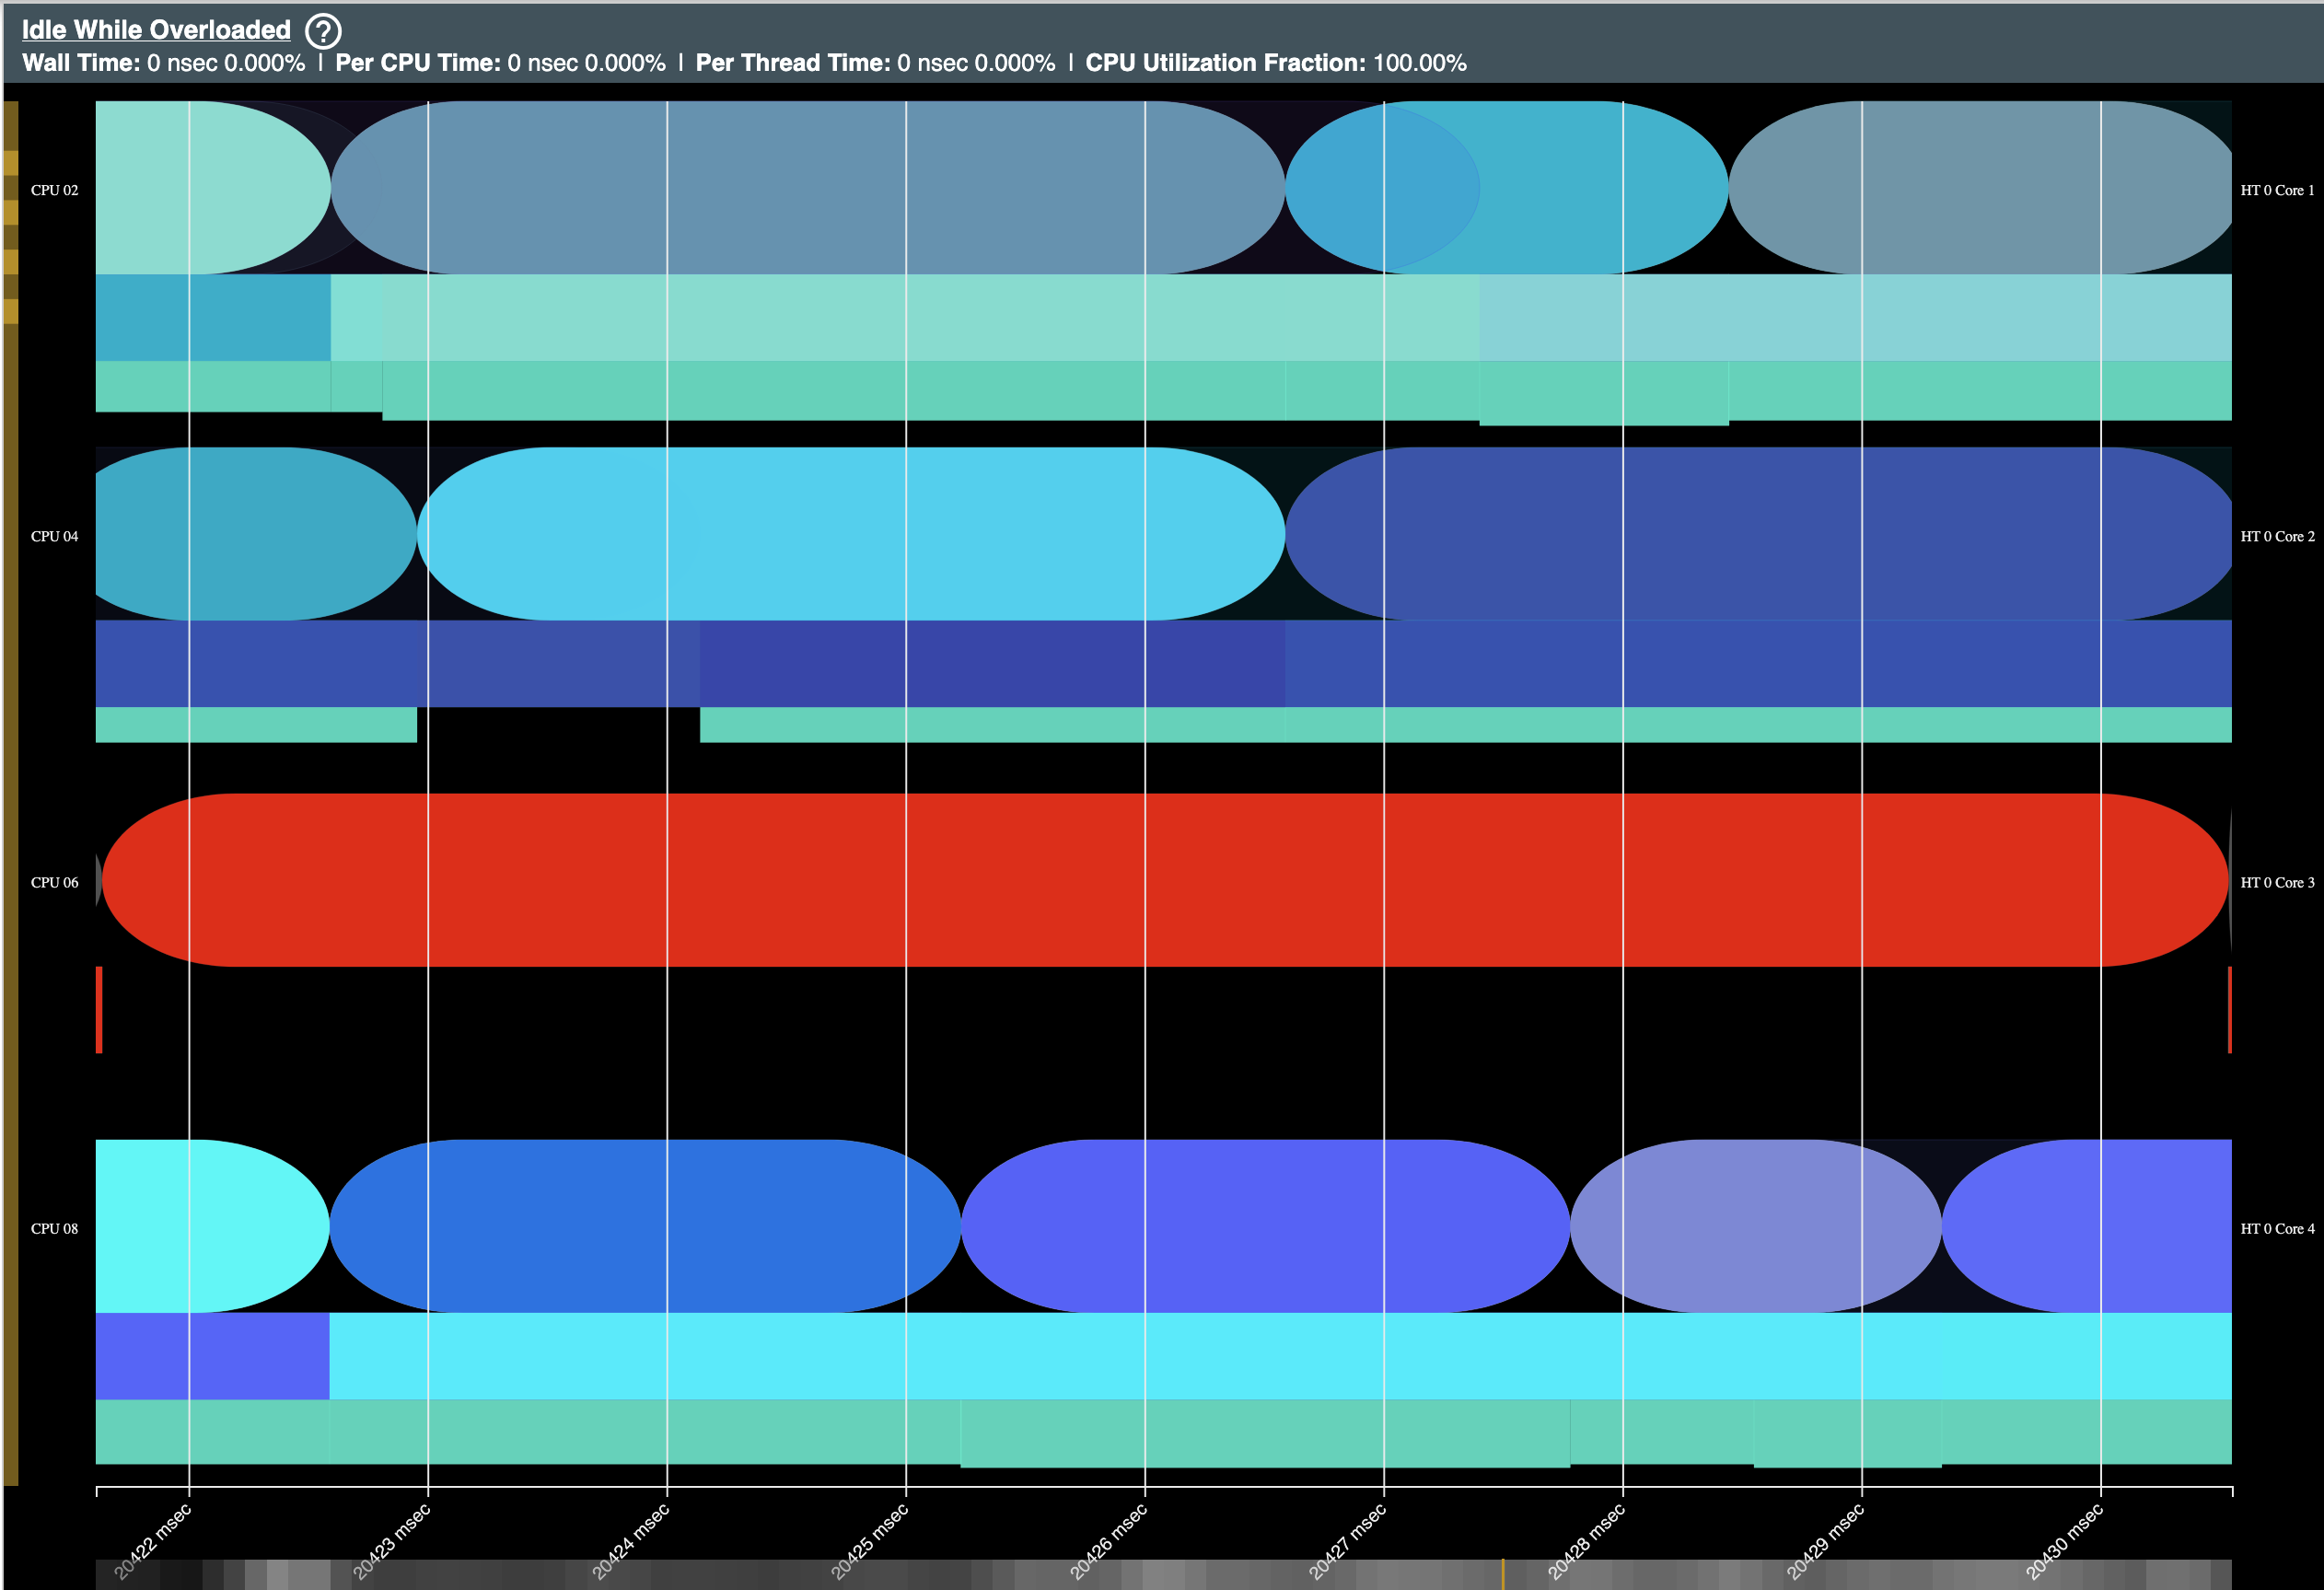
\includegraphics[width=\columnwidth]{graphs/schedviz-problem.png}
    \caption{Each thread is a different color. Circles represent which
    thread is running on that core, while rectangles underneath show waiting but
    runnable threads
    }\label{fig:schedviz-problem}
\end{figure}

The failure mode we observe is that \textit{one core is running a BE process,
while an LC process is waiting on another}. We analyze perf traces of the
scheduling decisions, and visualize the trace using schedviz~\cite{TODO}.
\autoref{fig:schedviz-problem} shows a 10ms outtake of the resulting image. The
process running on each core is shown as a an oval, and queued processes are
shown as rectangles below. The root of the undesirable behavior is: on core 6,
the red process that is running the whole time is a BE process, whereas LC
threads, shown in varying shades of blue, are queued on the other cores.

The reason this happens is that Linux maintains a separate runqueue on each
core, in order to avoid the synchronization overheads of accessing global state
for every scheduling decision. Within each runqueue, Linux does a pretty good
job of maintaining the correct ratio of received cputime; but it does not
enforce the weight ratios across cores. This leads to the above failure mode,
where one core has no runnable high weight processes and thus runs a low weight
one, whereas another core has queued high weight processes. This problem goes
away when there are no BE processes, because cores try to steal work before
going idle.

\subsection{This is not a bug}

The root of the problem goes deeper than just a poor implementation: a
weight-based interface is at odds with machine-wide policy enforcement. In
increasingly multi-core and multi-NUMA machines, synchronization is expensive.
This means that the overheads of maintaining global invariants can quickly
become prohibitive.

In order to strictly and globally enforce a processes weight, the scheduler
would need to synchronize at every scheduling decision: calculating whether a
given process is owed time globally requires knowing the total weight across all
cores as well as the sum of time that all the processes in the group have
gotten. At the same time, servers now have up to 8 NUMA nodes, and hundreds up
CPUs across them~\cite{TODO}. Synchronizing across them is expensive: in a
microbenchmark we found that even on a single NUMA node if each core takes a
lock to read the state on the other cores at every scheduling, this already
slows down the execution time of a simple cpu-bound loop by XX\%. This number
goes up to YY\% across two NUMA nodes. This is not surprising, other work has
also found that kernel lock contention is a bottleneck to performance at
scale~\cite{TODO}\hmng{the AFaaS cgroups pool thing here}


\subsection{The problems with weights add up}

\hmng{yes this section title is a pun, and yes I will be deleting it (jk jk\dots
unless\dots)}

\begin{figure}[t]
    \centering
    
\includegraphics[width=0.8\columnwidth]{graphs/todo.png}
    \caption{running the same experiment, with an increasing number of BE
    workloads}\label{fig:many-be}
\end{figure}

Using very large weight differentials as an interface to isolate LC and BE is
also bad for other reasons.

The first is that weights add up: although low weights run infrequently, they
still get a fair share, and in doing so impact the latency of the higher weight
(LC) processes. A large number of BE workloads each with a small weight adds up
to represent a significant amount of weight in the system, now contending
directly with the LC workload. We see this happen in a small microbenchmark, run
on one core in order to ensure a setting where we know Linux enforces weights
correctly.~\autoref{fig:many-be} shows the mean and 99th pctile latency increase
for the LC server when starting different numbers of BE workload, as compared to
an uncontended baseline. As expected, as the number of BE workloads goes up, the
impact on the latency of the LC server goes up. In fact, in order avoid this,
Kubernetes makes use of the nested structure of \cgroups{} to create a parent
group that gets a weight of 1 and holds all the best effort containers within
it.

The second reason that weights don't work as an interface to isolate LC from BE
is that the just discussed small fair share interacts with the scheduling tick
size. Barring other events such as blocking or wakeup, Linux only schedules
every hardware tick, which is usually 4ms. That means that when a BE processes'
turn to run does come around, it will interrupt any running LC process for
potentially a whole 4ms. This is a large amount of for microservice workloads,
whose SLOs are often in the low double digit or even single digit ms
realm.~\cite{TODO}




